\documentclass[aspectratio=169,10pt]{beamer}

% --- packages ---
\usepackage[utf8]{inputenc}
\usepackage[T1]{fontenc}
\usepackage{lmodern}
\usepackage{graphicx}
\usepackage{booktabs}
\usepackage{array}
\usepackage{xcolor}
\usepackage{hyperref}
\usepackage{multirow}

% --- theme ---
\usetheme{Madrid}
\usecolortheme{seahorse}
\setbeamertemplate{navigation symbols}{}
\setbeamertemplate{footline}[frame number]
\setbeamerfont{frametitle}{size=\large,series=\bfseries}
\setbeamerfont{footnote}{size=\tiny}

% --- semantic colors ---
\definecolor{good}{RGB}{21,127,59}
\definecolor{bad}{RGB}{176,0,32}
\definecolor{accent}{RGB}{26,61,124}
\newcommand{\good}[1]{\textcolor{good}{\textbf{#1}}}
\newcommand{\bad}[1]{\textcolor{bad}{\textbf{#1}}}
\newcommand{\dataset}[1]{\texttt{#1}}

% --- title ---
\title[Classical Threshold Generation for OBT]{Classical Threshold Generation\\ for Oblivious Trees}
\subtitle{Empirical study on the OBT pipeline --- results \& inferences}
\author[Poggiali, Berti]{Alessandro Poggiali \and Alessandro Berti}
\date{Variational Update --- April 2026}

\begin{document}

% =====================================================
\begin{frame}
  \titlepage
\end{frame}

% =====================================================
\begin{frame}{Context \& motivation}
  Building on the \textbf{Quantum Oblivious Trees} project, we paused the quantum
  direction to first \emph{understand the classical threshold-generation landscape}.

  \medskip
  The leaf-free, threshold-learning oblivious tree is novel even without quantum
  circuits --- it deserves a thorough classical study before layering quantum
  methods on top.

  \medskip
  \textbf{Why this matters.} The quantum circuit is just another \emph{indirect}
  parameterization of the thresholds. If indirect parameterization gives no
  advantage classically, the rationale for the quantum comparison must be
  re-stated.
\end{frame}

% =====================================================
\begin{frame}{Architecture recap}
  \begin{enumerate}
    \item A \textbf{threshold generator} outputs $d$ thresholds $t = \{t_1, \dots, t_d\}$ (one per tree level).
    \item Thresholds feed a \textbf{differentiable oblivious tree} $\rightarrow$ soft predictions $\hat{y}$ via sigmoid soft-binning + temperature annealing.
    \item \textbf{Leaves are computed empirically} (responsibility-weighted majority vote) --- not learned.
    \item BCE / CE loss $\mathcal{L}(y, \hat{y})$ $\rightarrow$ gradients flow back to the threshold generator.
    \item Generator parameters update; loop repeats. Sigmoid maps thresholds to $[0, 1]$.
  \end{enumerate}

  \medskip
  The generator takes a \emph{dummy input} --- no data encoding.
\end{frame}

% =====================================================
\begin{frame}{The two approaches under comparison}
  \centering
  \begin{tabular}{@{}lll@{}}
    \toprule
                       & \textbf{FFNN generator}                  & \textbf{Sampler}                                   \\
                       & ``CLASSICO FFNN''                        & ``CLASSICO SAMPLER''                               \\
    \midrule
    Threshold          & $t_i = \sigma(W \cdot x + b_i)$          & $t_i = \sigma(\theta_i),\ \theta_i \in \mathbb{R}$ \\
    Parameterization   & \textbf{Indirect} (network)              & \textbf{Direct} ($d$ learnable scalars)            \\
    Hypothesis         & more weights $\Rightarrow$ more expressive & minimal baseline                                 \\
    \# parameters      & $2d$ (0-layer) up to $\sim hd$ (1 hidden) & $d$                                                \\
    \bottomrule
  \end{tabular}

  \bigskip
  \begin{center}
    \emph{Question: does the indirect parameterization buy us anything?}
  \end{center}
\end{frame}

% =====================================================
\begin{frame}{Hypotheses we set out to test (Meeting 1)}
  \begin{enumerate}
    \item[\textbf{Q1.}] Is the FFNN necessary, or is direct optimization enough?
    \item[\textbf{Q2.}] Does adding hidden layers / neurons improve threshold quality?
    \item[\textbf{Q3.}] Convergence dynamics --- speed vs.\ final accuracy tradeoff?
    \item[\textbf{Q4.}] Optimizer / learning-rate sensitivity?
    \item[\textbf{Q5.}] How does the differentiable OBT compare to a standard sklearn DT?
  \end{enumerate}
\end{frame}

% =====================================================
\begin{frame}{Experimental design --- 4 studies}
  \centering
  \begin{tabular}{@{}clll@{}}
    \toprule
    \textbf{Study} & \textbf{Question}                  & \textbf{Sweep} \\
    \midrule
    1 & FFNN-0layer vs Sampler   & 22 datasets $\times$ \{FFNN-bias, FFNN-nobias, Sampler\} $\times$ depths \\
    2 & Effect of hidden layers  & 22 datasets $\times$ \{$h=4, 8, 16$\} $\times$ depths                    \\
    3 & Optimizer / LR sensitivity & \{Adam, SGD\} $\times$ \{0.001, 0.005, 0.01, 0.05, 0.1\}              \\
    4 & sklearn DT baseline      & 22 datasets, depth-matched DT                                            \\
    \bottomrule
  \end{tabular}

  \bigskip
  \begin{itemize}
    \item \textbf{Datasets:} 22 tabular classification datasets.
    \item \textbf{Metrics:} test accuracy, test CE, validation curves.
    \item \textbf{Multiple seeds} per config; mean $\pm$ std reported.
    \item \textbf{Total:} $171 + 171 + 1086 + 57 = \mathbf{1485}$ runs.
  \end{itemize}
\end{frame}

% =====================================================
\begin{frame}{Headline numbers}
  \centering
  \begin{tabular}{@{}cllcc@{}}
    \toprule
    \textbf{Study} & \textbf{Approach} & & \textbf{Test acc} & \textbf{\# params (avg)} \\
    \midrule
    1 & FFNN-0layer (bias)        & & 0.7046          & 14.5         \\
    1 & FFNN-0layer (no bias)     & & 0.7043          & 14.5         \\
    1 & \textbf{Sampler}          & & \good{0.7054}   & \good{7.3}   \\
    2 & FFNN-1h, $h=4$            & & 0.7053          & 44           \\
    2 & FFNN-1h, $h=8$            & & 0.7046          & 81           \\
    2 & FFNN-1h, $h=16$           & & 0.7047          & 155          \\
    3 & best (Adam, LR=0.01)      & & 0.7020          & ---          \\
    4 & \textbf{sklearn DecisionTree} & & \good{0.7129} & ---        \\
    \bottomrule
  \end{tabular}

  \bigskip
  All classical OBT variants are within \textbf{$\sim 0.001$} of each other.
  DT is \textbf{$\sim 0.8$\,pp} higher.
\end{frame}

% =====================================================
\begin{frame}{Inference 1 --- The FFNN is not necessary \hfill \small\textcolor{gray}{(Q1)}}
  \begin{itemize}
    \item Sampler and FFNN-0layer-no-bias are \emph{mathematically} near-equivalent given a 1-D dummy input --- $\sigma(w \cdot 1)$ is a reparameterized scalar.
    \item \textbf{Per-dataset accuracies are identical to 4 decimals on most datasets.}
    \item Sampler does this with \textbf{half the parameters} and one extra ``win'' overall.
  \end{itemize}

  \medskip
  \textbf{Bias term effect:} mean $+0.002$ (median $+0.001$), but $\pm 4$\,pp swings per dataset.
  \begin{itemize}
    \item Helps decisively on \dataset{led7} ($+0.11$), \dataset{car} ($+0.05$).
    \item Hurts on \dataset{australian} ($-0.08$), \dataset{ecoli} ($-0.06$), \dataset{heart} ($-0.05$).
    \item Net: a wash, not a real effect.
  \end{itemize}

  \medskip
  \begin{block}{Take-away}
    Indirect FFNN parameterization buys \textbf{nothing} over a direct learnable parameter.
    The ``more weights $\Rightarrow$ more expressive thresholds'' hypothesis \textbf{does not hold}.
  \end{block}
\end{frame}

% =====================================================
\begin{frame}{Inference 2 --- Hidden layers don't help either \hfill \small\textcolor{gray}{(Q2)}}
  \centering
  \begin{tabular}{@{}lcc@{}}
    \toprule
    \textbf{Config} & \textbf{\# params} & \textbf{Mean test acc} \\
    \midrule
    0-layer        & 14  & 0.7046 \\
    1 hidden, $h=4$  & 44  & 0.7053 \\
    1 hidden, $h=8$  & 81  & 0.7046 \\
    1 hidden, $h=16$ & 155 & 0.7047 \\
    \bottomrule
  \end{tabular}

  \medskip
  \begin{flushleft}
    Going from \textbf{14 $\rightarrow$ 155} parameters yields a delta of \textbf{$+0.0001$} in mean test accuracy.

    The 18-vs-4 win-count for $h=16$ is rounding noise.
  \end{flushleft}

  \medskip
  \begin{block}{Take-away}
    The expressiveness bottleneck is \textbf{not} in the threshold generator.
    Whatever blocks further accuracy lives in the \textbf{differentiable oblivious tree itself}
    --- soft binning, leaf computation, temperature schedule --- not in how thresholds are produced.
  \end{block}
\end{frame}

% =====================================================
\begin{frame}{Inference 3 --- Convergence dynamics \hfill \small\textcolor{gray}{(Q3)}}
  \centering
  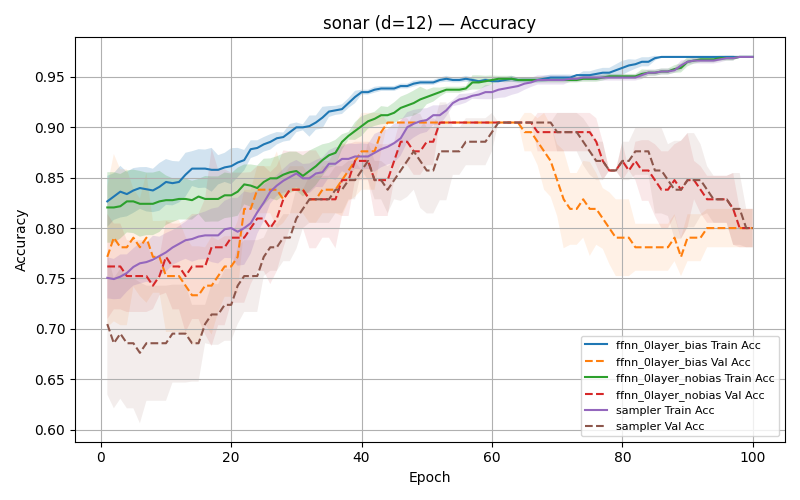
\includegraphics[width=0.48\linewidth]{../results/study1/plots/sonar/convergence_acc_d12.png}\hfill
  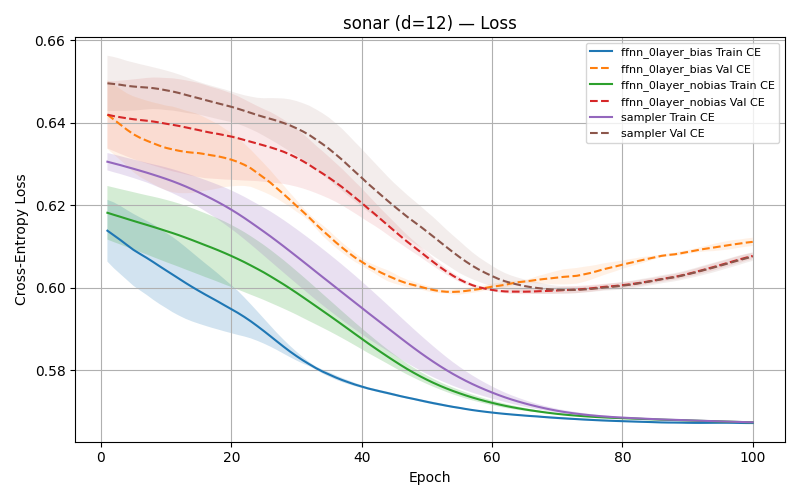
\includegraphics[width=0.48\linewidth]{../results/study1/plots/sonar/convergence_loss_d12.png}

  \scriptsize \dataset{sonar}, depth $= 12$. Final accuracy is \textbf{tied}, but the dynamics differ.

  \normalsize
  \begin{itemize}
    \item \textbf{FFNN-bias} starts higher, reaches its plateau \textbf{$\sim$30 epochs faster}.
    \item \textbf{Sampler} trains slowest, ends at the same point.
    \item FFNN validation \textbf{oscillates and degrades} after $\sim$60 epochs (overfitting visible).
    \item Sampler's validation is \textbf{smoother} and more stable.
  \end{itemize}

  \medskip
  \emph{Same destination, different path: FFNN is faster but more variance / overfitting; Sampler is slower but better-behaved.}
\end{frame}

% =====================================================
\begin{frame}{Inference 4 --- Optimizer / LR sensitivity \hfill \small\textcolor{gray}{(Q4)}}
  \centering
  \begin{tabular}{@{}llcc c@{}}
    \toprule
                       & \textbf{best LR} & \textbf{best acc} & \textbf{spread (max $-$ min)} \\
    \midrule
    FFNN, \textbf{Adam}    & 0.01 & 0.7020 & 0.013 \\
    FFNN, SGD              & 0.10 & 0.6760 & 0.022 \\
    Sampler, \textbf{Adam} & 0.01 & 0.7019 & 0.023 \\
    Sampler, SGD           & 0.10 & 0.6664 & 0.018 \\
    \bottomrule
  \end{tabular}

  \bigskip
  \begin{itemize}
    \item \textbf{Adam strictly dominates SGD} by $\sim$3\,pp regardless of approach. SGD never catches up, even at LR=0.1.
    \item \textbf{Sampler is $\sim 2\times$ more LR-sensitive} under Adam --- drops to 0.679 at LR=0.001 while FFNN holds 0.689.
    \item \textbf{Adam @ LR=0.01} is the safe default for both.
  \end{itemize}
\end{frame}

% =====================================================
\begin{frame}{Inference 5 --- DT baseline reveals an OBT failure mode \hfill \small\textcolor{gray}{(Q5)}}
  Per-dataset head-to-head (best Study-1 OBT vs sklearn DT, averaged over depths):

  \begin{itemize}
    \item \textbf{OBT wins 14/22}, DT wins 8/22. Mean diff $+0.012$ in favor of OBT.
    \item But DT \emph{crushes} OBT on a \textbf{specific cluster of datasets}:
  \end{itemize}

  \centering
  \begin{tabular}{@{}lcl@{}}
    \toprule
    \textbf{Dataset}    & \textbf{OBT $-$ DT} & \textbf{Notes} \\
    \midrule
    \dataset{avila}     & \bad{$-0.26$} & OBT stuck at 0.411 ($\approx$ majority class) at \emph{every} depth \\
    \dataset{egg}       & \bad{$-0.19$} & OBT stuck at 0.567 at every depth                                  \\
    \dataset{drybean}   & $-0.09$       & OBT improves with depth, DT just better                            \\
    \dataset{car}       & $-0.08$       &                                                                    \\
    \dataset{glass}     & $-0.06$       &                                                                    \\
    \bottomrule
  \end{tabular}

  \medskip
  \footnotesize
  OBT crushes DT on \dataset{sonar} ($+0.18$), \dataset{australian} ($+0.14$), \dataset{lymph} ($+0.14$),
  \dataset{yeast} ($+0.11$), \dataset{pima} ($+0.10$), \dataset{heart} ($+0.09$), \dataset{iris} ($+0.08$),
  \dataset{fico} ($+0.06$).
\end{frame}

% =====================================================
\begin{frame}{Inference 5 --- what \texttt{avila} and \texttt{egg} look like}
  \centering
  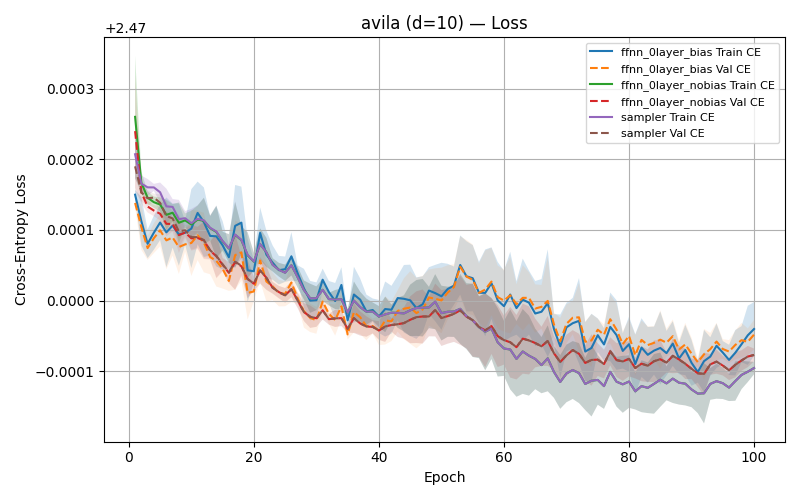
\includegraphics[width=0.48\linewidth]{../results/study1/plots/avila/convergence_loss_d10.png}\hfill
  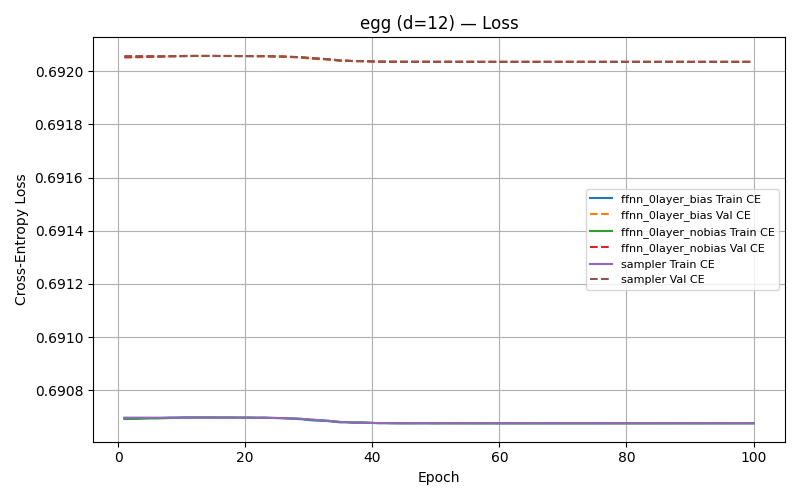
\includegraphics[width=0.48\linewidth]{../results/study1/plots/egg/convergence_loss_d12.png}

  \scriptsize CE loss barely moves on \dataset{avila} ($2.4707 \rightarrow 2.4699$ over 100 epochs)
  and \dataset{egg} --- for \emph{every} classical OBT variant: FFNN-bias, FFNN-nobias, Sampler, $h=4/8/16$.

  \normalsize
  \medskip
  \begin{block}{Pattern}
    OBT wins on \textbf{binary / well-separated} datasets, loses on \textbf{multi-class}
    problems where greedy splitting matters. The collapse to majority-class is a
    \textbf{soft-binning landscape failure}, not a threshold-generator failure.
  \end{block}
\end{frame}

% =====================================================
\begin{frame}{Hidden layers don't rescue \texttt{avila} either}
  \centering
  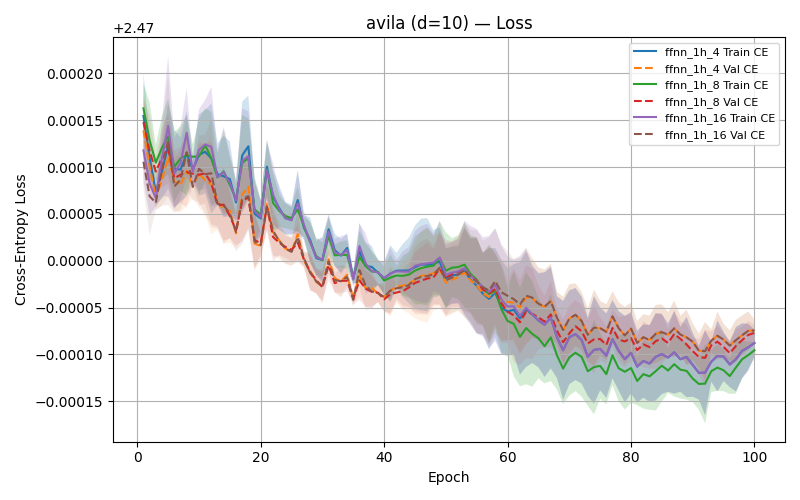
\includegraphics[width=0.62\linewidth]{../results/study2/plots/avila/convergence_loss_d10.png}

  \medskip
  \scriptsize Study 2, \dataset{avila}, depth $= 10$. $h=4$, $h=8$, $h=16$ all flatline at the same loss
  --- confirms the bottleneck is downstream of the threshold generator.
\end{frame}

% =====================================================
\begin{frame}{What this means for the project}
  \begin{enumerate}
    \item \textbf{For the classical study.} Keep the cheapest baseline: \textbf{Sampler}.
          FFNN adds parameters and overfitting risk for \textbf{zero} accuracy gain.
          Hidden layers can be dropped from future grids.
    \item \textbf{For the quantum direction.} The ``indirect parameterization buys expressiveness''
          rationale that motivated the quantum comparison \textbf{didn't survive the classical ablation}.
          A quantum threshold generator must demonstrate something \emph{other than}
          expressive thresholds --- e.g.:
          \begin{itemize}
            \item better optimization landscape,
            \item robustness on hard datasets (\dataset{avila}, \dataset{egg}),
            \item different inductive bias.
          \end{itemize}
    \item \textbf{The most interesting open problem} is \emph{not} FFNN-vs-Sampler-vs-Quantum.
          It is:
          \begin{quote}
            \emph{Why does the soft-OBT collapse to majority-class on \dataset{avila} and \dataset{egg}
            regardless of who generates the thresholds?}
          \end{quote}
          Worth investigating before pouring more cycles into threshold generators.
  \end{enumerate}
\end{frame}

% =====================================================
\begin{frame}{Why is this the most interesting question?}
  \begin{enumerate}
    \item \textbf{It is the actual bottleneck.} Studies 1--2 ruled out the threshold
          generator (Sampler $\approx$ FFNN-0layer $\approx$ FFNN-1h within $\sim 0.001$);
          Study 3 ruled out optimizer / LR. All those interventions live \emph{upstream}
          of where \dataset{avila} / \dataset{egg} fail $\Rightarrow$ the failure must live
          in the soft-OBT layer itself.
    \item \textbf{It re-frames the quantum question} --- the whole point of the broader project.
          The classical ablation killed the ``expressive thresholds'' rationale. If a quantum
          generator is to add value, this finding tells us \emph{where the room actually is}:
          the optimization landscape / inductive bias of the OBT layer, not threshold expressiveness.
    \item \textbf{Sharp, falsifiable empirical signature.} On \dataset{avila}, CE loss moves
          $2.4707 \rightarrow 2.4699$ over 100 epochs, across \emph{every} generator variant
          and \emph{every} depth --- while \dataset{sonar} / \dataset{iris} train fine.
          Two clean regimes from the same architecture $\Rightarrow$ tractable to diagnose
          (loss-landscape probe, gradient-norm analysis, temperature ablation).
    \item \textbf{A class of failure, not a quirk.} Losing cluster
          (\dataset{avila}, \dataset{egg}, \dataset{drybean}, \dataset{car}, \dataset{glass})
          is \emph{multi-class}; winning cluster is binary / well-separated. The pattern likely
          generalizes to other soft-decision models (NODE, soft trees).
    \item \textbf{Opportunity cost.} Generator-vs-generator competition is now bounded above
          by $\sim 0.001$ in mean accuracy. Fixing \dataset{avila} alone is bounded above by
          \textbf{$+0.26$ on a single dataset}. That is where the cycles pay off.
  \end{enumerate}
\end{frame}

% =====================================================
\begin{frame}{Proposed next steps}
  \begin{itemize}
    \item \textbf{Diagnose the soft-binning failure} on \dataset{avila} / \dataset{egg}:
          \begin{itemize}
            \item loss-landscape inspection at the OBT layer (not the generator),
            \item temperature-schedule ablation; revisit annealing,
            \item leaf-computation alternatives (responsibility-weighting variants).
          \end{itemize}
    \item \textbf{Drop FFNN from the grid}; promote Sampler as the classical reference.
    \item \textbf{Re-frame the quantum question}: target \emph{optimization landscape} or
          \emph{inductive bias}, not threshold expressiveness.
    \item \textbf{Multi-class focus}: a sub-grid of multi-class datasets to track the OBT
          failure mode under interventions.
  \end{itemize}
\end{frame}

\end{document}
